% Standalone section fragment for the structural-modeling chapter.
\section{构建扭转双层}\label{sec:twisted-structures}
\index{Niuzhuan shuangceng@扭转双层}
\index{Moer chaojingge@莫尔超晶格}

\subsection{从相对转角到共同周期}

将两张石墨烯单层重叠，再使其中一层绕法向转动，局部的原子对齐关系就会随位置改变：有些区域接近原子上下相对，有些区域接近一层原子落在另一层六元环中心。把视野扩大，可以看到这些局部排列组成较大的重复图案，称为莫尔图案。

用于周期计算的模型还需要一个共同晶胞。上层不能只在原来的小晶胞中任意旋转，否则越过晶胞边界后，两层的排列通常接不上。\ui{扭转莫尔超晶格}为两层分别选择整数超胞，使它们能够放入同一面内周期。输入的目标角用于寻找合适的匹配，最终模型则由一组具体的整数关系确定。

本节使用约 $21.7868^\circ$ 的石墨烯双层作为第一例。这个转角对应较小的共同周期，结果只有 28 个碳位点，便于同时观察两层和晶胞。先完成这个例子，再尝试较小转角，能够更清楚地理解角度、周期和模型规模之间的关系。

\subsection{准备上下两层}

本工具使用六方面内原胞：两个面内晶格矢量等长，夹角为 $60^\circ$ 或 $120^\circ$。本例的单层石墨烯包含两个 C 位点，面内晶格常数为 $2.46\,\text{\AA}$，盒高为 $15\,\text{\AA}$。两个面内方向周期重复，法向为非周期。

随书的\file{twist-graphene-bottom.json}与\file{twist-graphene-top.json}来自同一份单层输入，分别供底层和上层使用。它们与前面\file{graphene-layer.json}的几何相同。两份文件分开命名，是为了让项目中的角色一目了然，不表示两层已具有不同转角。

\begin{steps}
  \item 把两份 JSON 导入同一项目，分别将结构命名为\file{twist-bottom}和\file{twist-top}。
  \item 打开底层的三维文档，检查它只有两个模型位点。屏幕上用于显示周期连接的映像原子可以多于两个。
  \item 查看晶格，确认面内长度均为 $2.46\,\text{\AA}$、夹角约为 $120^\circ$。再检查上层具有相同的晶格和组成。
  \item 激活\file{twist-bottom}。在顶部\ui{晶体建模}的\ui{表面与界面}区域打开\ui{界面建模}，选择\ui{扭转莫尔超晶格}。
  \item 在\ui{上层结构}下拉菜单中选择\file{twist-top}。这里选的是项目中已有的结构，不是在输入框中填写磁盘路径。
\end{steps}

第一次练习应从这两张原始单层开始。前面已经插入或堆叠过的双层可另行保留，不能再把它当成一张原始单层送入本例。

\subsection{填写一组小规模参数}

\begin{table}[htbp]
\centering
\caption{28位点石墨烯扭转双层的练习参数。}
\begin{tabularx}{\linewidth}{lX}
\toprule
参数 & 本例输入与含义\\
\midrule
上层结构 & 在下拉菜单中选择\file{twist-top}。\\
角度（度） & 输入\literalinput{21.786789}，作为目标相对转角。\\
层间距（Å） & 输入 3.35，规定两张单层之间的初始间隔。\\
总真空层厚度（Å） & 输入 15，规定薄片之外的总空白高度。\\
允许的最大面内应变 & 输入 0.03，即 3\%。\\
最大原子数 & 输入 200，限制生成模型的总位点规模。\\
最大周期匹配指数 & 输入 6，限定本次整数匹配的搜索范围。\\
\bottomrule
\end{tabularx}
\end{table}

\ui{角度（度）}是一个数值框，输入的是度数；不需要再写度符号。\ui{层间距}和\ui{总真空层厚度}也都是长度数值。最大应变则是比例，0.03 表示 3\%，不能把 3 直接填作同一个要求。

最大原子数不是要求软件一定生成 200 个原子，而是允许的上限。最大周期匹配指数也不是沿某个方向简单重复 6 次。工具会在这个范围内寻找整数匹配，综合考虑目标角偏差、应变和结构大小，再选出一组结果。因此，这两个上限与\ui{构建超胞}中的三个重复倍数有不同含义。

本命令内部选择一组匹配，不提供\ui{堆叠异质结构}那样的候选排序和候选序号字段。填写完参数后，应检查生成结构的实际规模和相对取向；需要比较其他匹配时，保留原始两层，分别生成和保存各组参数的结果。

\begin{steps}
  \item 按表填写参数，先使用\ui{预览}检查。模型应从两个位点的单层变成两层组成的较大周期结构。
  \item 沿接近表面法向观察，检查两层的六元环排列已经相对转动；转到侧面，确认仍然只有两层，层间没有意外插入其他原子。
  \item 检查模型位点总数应为 28。面内晶胞扩大后，查看器的显示映像数仍可能多于这个数。
  \item 应用后把结果命名为\file{graphene-twist-21p786789}，保存项目。保留两份输入单层，使后续比较可以从同一起点开始。
\end{steps}

\begin{figure}[H]
\centering
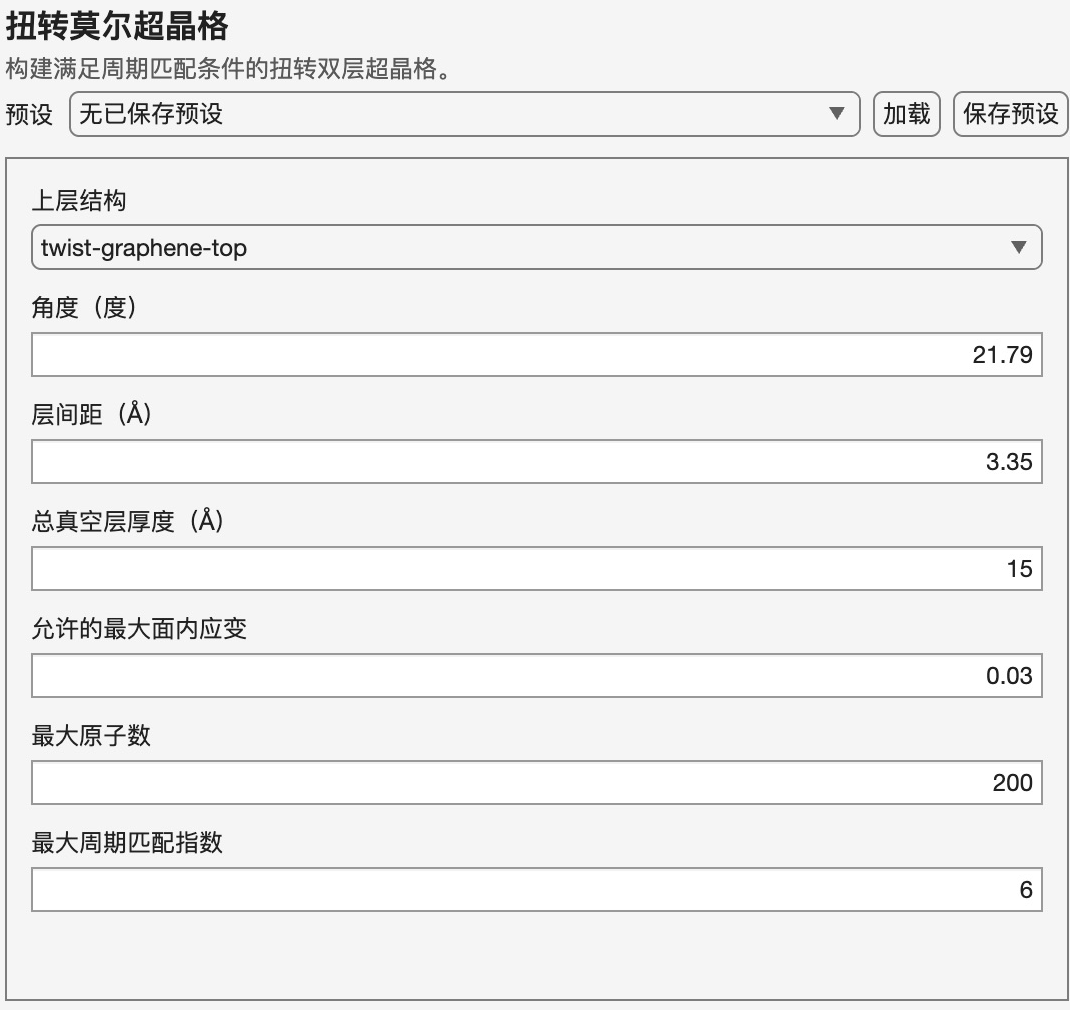
\includegraphics[width=107mm]{publication-assets/crop-7c221ceb9a35fdad53a3.png}
\par\vspace{2mm}

\includegraphics[width=60mm]{publication-assets/crop-faecdf5879e359505e34.png}
\caption{扭转参数与预览提示，尚未应用。本次输入目标角21.786789度；数值框失去焦点后按显示精度呈现为21.79。上层在图中保留导入时的名称\file{twist-graphene-top}，对应本节的\file{twist-top}；预览生成28个位点。}
\label{fig:online-twist-parameters}
\end{figure}

\begin{figure}[H]
\centering
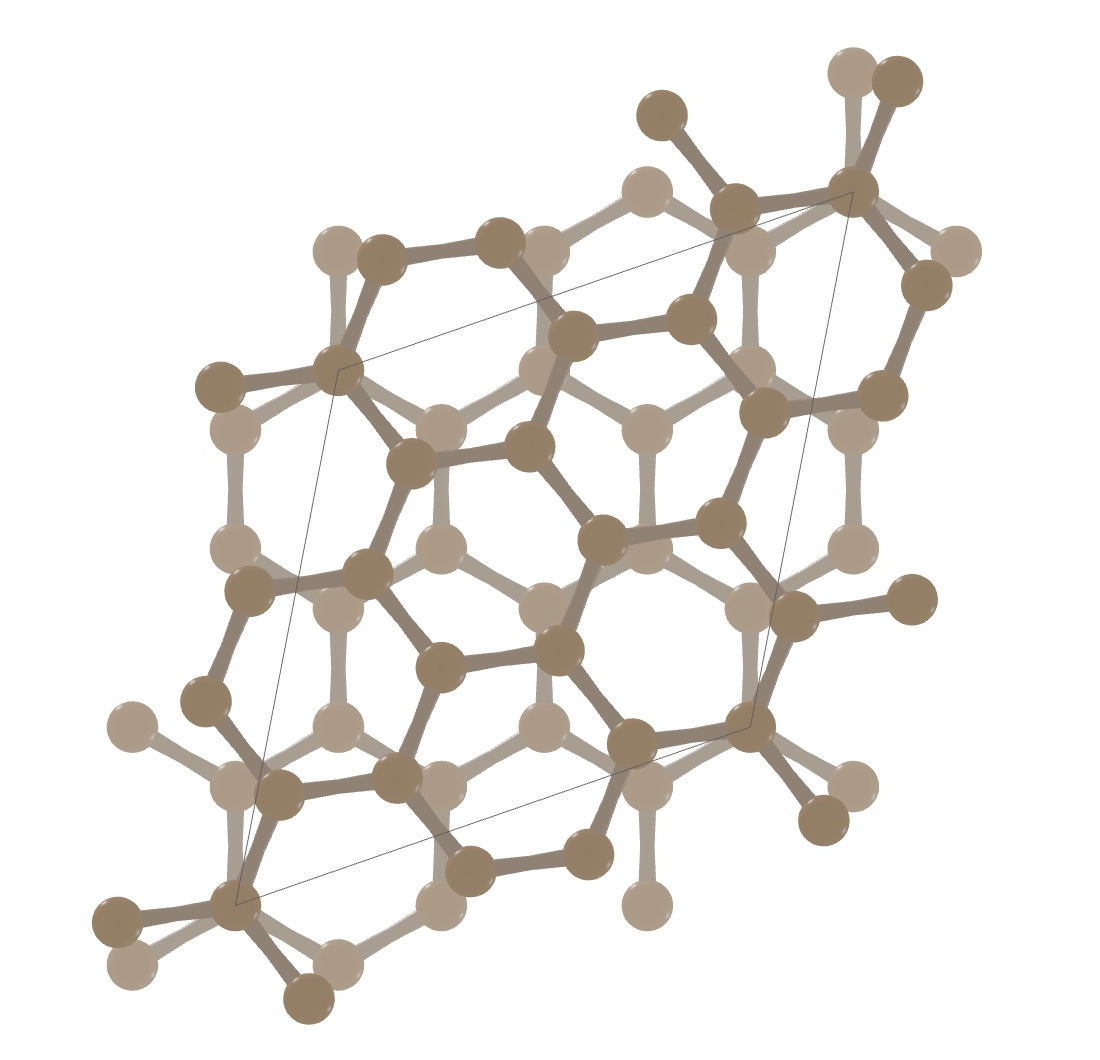
\includegraphics[width=93mm]{publication-assets/crop-89eb072a4598add87b05.png}
\caption{石墨烯扭转双层的法向视图。两层的六元环相对转动；28个模型位点按当前周期范围显示为68个原子。}
\label{fig:online-twist-top}
\end{figure}

\subsection{读懂生成的晶胞}

随书\file{graphene-twist-21p786789.json}是按上述参数得到的参考结构，另提供几何交换用的同名 CIF。模型有 28 个 C 位点，分为两层，每层 14 个。与原始每层两个位点相比，每一层的面内面积扩大为原来的 7 倍。

面内两个晶格矢量等长，均约为 $6.508548\,\text{\AA}$。相应面积约为 $36.6859\,\text{\AA}^2$。本例的新面内夹角为 $60^\circ$；输入原胞的夹角为 $120^\circ$，两者是不同的晶格基底表示，不能只凭角度改变就判断晶体被拉歪。核对长度、面积、位点数与两层的周期连接，应当放在一起进行。

对于这组石墨烯输入，周期边长也可用 $\sqrt{7}\times2.46\,\text{\AA}$ 核对，约为 $0.651\,\mathrm{nm}$。这里的周期描述共同晶胞在面内的重复长度，不是层间距离，也不是某条 C--C 键长。模型中每层最短近邻距离仍约为 $1.420282\,\text{\AA}$，与输入单层一致。

从侧面看，两层相隔 $3.35\,\text{\AA}$，法向胞高为 $18.35\,\text{\AA}$。这组模型中每层原子各在一个平面内，所以本例胞高等于层间距与总真空之和。总真空 $15\,\text{\AA}$ 是整个薄片之外的空白高度；它不表示薄片上方和下方各有 $15\,\text{\AA}$。

\begin{figure}[H]
\centering
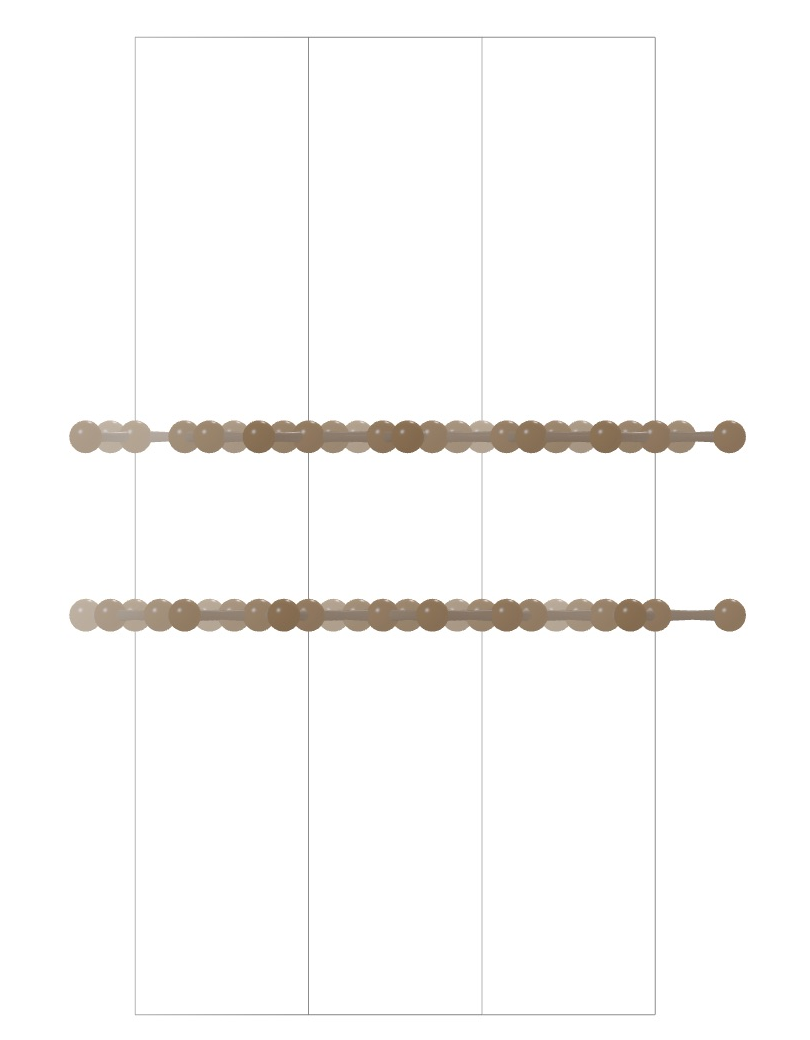
\includegraphics[width=67mm]{publication-assets/crop-a8d161a93e2745b16ef3.png}
\caption{同一模型的侧视。两张原子平面与法向晶胞边界一起显示，便于分辨层间距离和外侧真空。}
\label{fig:online-twist-side}
\end{figure}

随书参考结构的实际匹配角为 $21.786789298^\circ$，与目标角相差约 $2.98\times10^{-7}$ 度，面内应变为 0。几何核对还分别提取两层近邻键的方向，得到相同的相对角度。因此，确认扭转结构时既要读匹配信息，也要检查原子的实际排列。

精确的角度和匹配信息保存在原生 JSON 的\file{properties}下的\file{moire}部分。用普通文本编辑器打开本例 JSON，搜索\file{achieved_angle_degrees}即可找到实际角；\file{target_angle_degrees}是目标角，\file{angle_error_degrees}是两者的偏差，\file{in_plane_strain}是面内应变。对自己生成的结构，在查看器的\ui{Export file}中选择\ui{Structure file}，再选 JSON 导出。不应选择同一菜单里的\ui{Scene JSON}，后者保存查看场景，不能用来查找上述结构匹配信息。

\subsection{目标角与实际角为什么可能不同}

目标角的输入范围为 $0^\circ$ 到 $60^\circ$。按六方面内晶格的对称关系，工具把实际匹配角表示在 $0^\circ$ 到 $30^\circ$ 之间；比较较大目标角时，也应按这一表示约定查看结果。本节先在这个较小范围内练习，便于直接比较目标值与实际值。

共同周期只能由特定整数关系构成。输入一个任意小数角，并不意味着一定存在大小合适、又完全等于该角的周期胞。本例把目标改成 $22^\circ$，保持其他参数不变，仍然得到 28 位点结构，实际角仍约为 $21.786789298^\circ$，角度偏差约为 $0.213211^\circ$。

这两次构建具有相同的最终几何，却对应不同的目标输入。随书\file{graphene-twist-target22.json}保留了第二次结果，便于比较。报告模型时，应记录实际角，而不是只把参数窗口中输入的目标角写进图题。

\begin{table}[htbp]
\centering
\caption{本组输入下目标角与规模限制的实际对照。}
\begin{tabularx}{\linewidth}{lX}
\toprule
输入变化 & 实际生成结果\\
\midrule
目标 $21.786789^\circ$，上限200 & 28位点，实际约 $21.786789298^\circ$。\\
目标 $22^\circ$，上限200 & 仍为28位点和同一实际角，偏差约 $0.213211^\circ$。\\
目标 $21.786789^\circ$，上限24 & 本例选择4位点、接近 $0^\circ$ 的匹配，未达到原目标。\\
\bottomrule
\end{tabularx}
\end{table}

第三行说明，完成构建与达到目标角是两项不同的检查。28位点的匹配被上限24排除后，工具会在剩余范围内选择结果。构建后，看到数量与预期明显不同，应回到参数和实际角一起核对，再决定是否增大搜索范围。

较小转角通常需要较长的共同周期和更多原子。比较不同转角时，可以先固定层间距与应变要求，再逐步增加允许的模型规模和匹配指数。这样更容易看清新增的搜索范围究竟改善了角度匹配，还是只带来更大的结构。本节约 $21.8^\circ$ 的例子使用较小整数，适合作为操作和周期检查的起点。

\subsection{按研究目的选择组装入口}

\ui{界面建模}菜单把几种组装方式放在一起。选择时，先明确已经知道哪些几何关系，再决定让工具寻找什么。

\begin{table}[htbp]
\centering
\caption{直接插入、层匹配与扭转构建的选择。}
\begin{tabularx}{\linewidth}{lX}
\toprule
入口 & 适合开始的情形\\
\midrule
插入结构 & 两部分的位置已经确定，只需给出相对平移；保留当前宿主晶胞。\\
堆叠异质结构 & 希望比较共同面内晶胞，从允许应变、重复范围与旋转范围中选择候选。\\
扭转莫尔超晶格 & 已有六方单层和目标转角，希望寻找相应的整数共同周期。\\
\bottomrule
\end{tabularx}
\end{table}

在\ui{堆叠异质结构}的候选表中，面积、应变、原子数和旋转角各自回答不同问题。面积与原子数反映计算规模；应变说明原始晶格需要改变多少才能匹配；旋转角说明两层如何相对定向。应变很小的候选也可能很大，面积最小的候选也可能需要较大形变。先比较这些量，再看具体原子排列，选择会更有依据。

本节的扭转命令则先利用六方整数关系确定一组共同周期，再组装两层。它不会要求在同一个窗口中填写\ui{候选序号}。如果希望比较目标 $21.786789^\circ$ 与 $22^\circ$，应分别从两张原始单层构建，分别记录结果，而不是在前一个已完成的双层上再次施加相同命令。

同样，直接旋转屏幕上的观察方向只会改变视角；选择一组原子进行旋转则改变原子位置。两者都不能代替共同晶胞的周期匹配。检查扭转模型时，除观察两层取向，还应显示晶胞边框，沿两个面内方向查看重复后的连接，确认局部图案与整个周期表达的是同一模型。

如果研究对象是面内并排相接的两种材料，而不是沿法向叠放的两层，本节的层间距和上下层组装并不描述那种几何关系。当前这组入口建立的是层状界面；描述面内结区时，应另外准备相应的原子排列与边界，不能只把上层名称换成第二种材料便当作完成了面内异质结。

\subsection{进一步建立石墨烯/h-\headinglatin{BN}扭转异质结构}

扭转不只用于同一种材料的双层。前面石墨烯与 h-BN 的零转角匹配，主要展示两种面内晶格常数如何协调；在此基础上，还可以同时引入相对转角。本例仍使用石墨烯作为底层，h-BN 作为上层：石墨烯晶格常数为 $2.46\,\text{\AA}$，h-BN 为 $2.50\,\text{\AA}$。

\begin{steps}
  \item 重新导入\file{twist-graphene-bottom.json}与\file{hBN-layer.json}，分别命名为\file{graphene-bottom}和\file{hBN-top}。不要把前一个已经扭转的双层作为底层。
  \item 激活新的石墨烯单层，在\ui{扭转莫尔超晶格}中将\ui{上层结构}选择为\file{hBN-top}。
  \item 沿用表中的目标角、层间距、总真空、200位点上限与匹配指数6，允许最大面内应变仍设为0.03。
  \item 预览后核对组成应为 $\mathrm{C_{14}B_7N_7}$，共28个位点。上层和底层各有14个位点，但元素组成不同。
  \item 应用并保存为\file{graphene-hBN-twist-21p786789}，再与零转角的\file{graphene-hBN-stacked.json}比较。
\end{steps}

本次实际角同样约为 $21.786789298^\circ$，面内主应变为 0.016，即 1.6\%。h-BN 的面内尺寸被匹配到石墨烯共同晶格，层间距仍为 $3.35\,\text{\AA}$，法向胞高仍为 $18.35\,\text{\AA}$。应变和转角描述的是不同变化：前者调整尺寸，后者改变两层的相对方向。

两种构建命令得到的都是几何模型。研究界面电荷转移、能带对齐或结区性质时，需要在保存的结构上继续建立相应计算，并区分构建输入的层间距与计算后得到的距离。

\subsection{保存扭转模型}

保存项目可以保留输入层、生成结构和后续工作流。单独交换结构时，本组提供 JSON 与 CIF 两种格式：JSON保留面内/法向周期标记、层编号和扭转匹配信息；CIF便于交换晶胞与原子位置。当前读回本组CIF时，三个方向均按周期处理，且不会保留莫尔匹配元数据。继续本章的二维建模比较，优先使用JSON；使用CIF进入其他计算流程时，再按目标方法确认法向边界与真空设置。

\begin{steps}
  \item 为每个结果写清材料、实际角和主要变化，例如“石墨烯双层，实际21.7868度”，不要只保存\file{result}之类的通用名称。
  \item 记录输入层的晶格、目标角与实际角、应变、层间距、总真空、位点数及面内周期。比较表可将这些量各占一列。
  \item 保存项目后重新打开，再检查上下两层的组成和晶胞。导出结构时，保留对应的参数记录，便于解释另一个软件中看到的模型。
  \item 需要重复生成时，在以\file{-nojvm}启动的完整 MATLAB\regmark{} 会话中，配置好工具箱路径后，从本手册仓库根目录运行随书\file{twist_examples.m}；只检查已保存文件时，运行\file{verify_twist_examples.m}。
\end{steps}

随书结构提供未作电子结构计算和层间弛豫的几何起点。生成与重新导入核对方法见配套脚本。后续比较扭角效应时，应把相同的泛函、赝势、截断能和合适的采样条件与这些几何记录一起保存，使每一张结果图都能找到对应的结构和计算条件。
